\documentclass[reqno, 12pt]{amsart}

\usepackage{amssymb, amsmath, amsthm, enumerate, mathtools, graphicx, enumitem, tikz, color, soul, bbm, verbatim, parskip, multicol}
\usepackage[margin=1 in]{geometry}
\usepackage[mathscr]{euscript}
\usepackage[urlcolor=blue,colorlinks=true]{hyperref}
\setlist[itemize]{noitemsep, topsep=0pt, parsep=0pt, partopsep=0pt}
\allowdisplaybreaks

\newcommand{\R}{\mathbb R}
\newcommand{\proj}{\operatorname{proj}}


%%%%%%%%%%%%%%%%%%%%%%%%%%%%%%%%%%%%%
\usepackage{mdframed}
\newmdenv[
  linewidth=1pt,
  linecolor=black,
  topline=true,
  bottomline=true,
  leftline=true,
  rightline=true,
  innertopmargin=10pt,
  innerbottommargin=10pt,
  innerleftmargin=10pt,
  innerrightmargin=10pt
]{answerbox}

\usepackage{pgfplots}
\pgfplotsset{compat=1.18}
\usepgfplotslibrary{fillbetween}
%%%%%%%%%%%%%%%%%%%%%%%%%%%%%%%%%%%%%


\pagestyle{plain}


\begin{document}

\begin{center}
  {\bf MATH 231-01: Homework Assignment 8}\\~\\
  3 November 2025\\~\\~\\~\\~\\~\\
\end{center}

{\bf Due:} 10 November 2025 by 10:00pm Eastern time, submitted on Moodle as a single PDF.~\\


{\bf Instructions:} Write your solutions on the following pages. If you need more space, you may add pages, but make sure they are in order and label the problem number(s) clearly. You should attempt each problem on scrap paper first, before writing your solution here. Excessively messy or illegible work will not be graded. You must show your work/reasoning to receive credit. You do not need to include every minute detail; however the process by which you reached your answer should be evident. You may work with other students, but please write your solutions in your own words.

~\\~\\~\\~\\~\\
{\bf Name:} Sean Balbale

~\\
{\bf Score:}

\newpage
\begin{itemize}

  \item[1.] Find the volume of the region that lies above the solid triangle with vertices $(0,0,0)$, $(1,0,0)$, $(1,2,0)$ and below the paraboloid $z = 6-x^2-y^2$.
    \newline

    \begin{answerbox}

      \begin{enumerate}
        \item First, sketch the region of integration in the $xyz$-plane.
          \begin{center}
            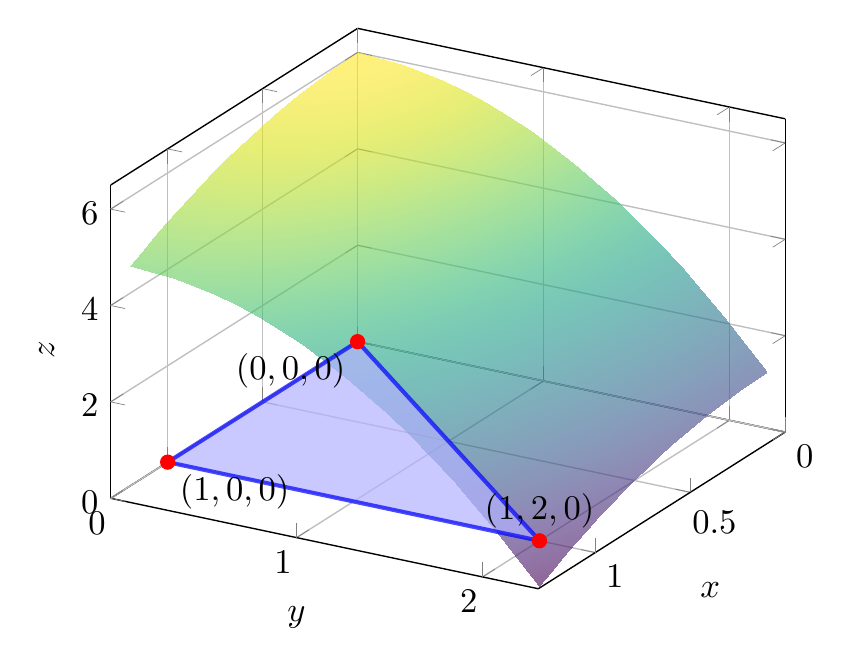
\begin{tikzpicture}[scale=1.25]
              % Define the paraboloid surface
              \begin{axis}[
                  view={120}{30},
                  xlabel=$x$,
                  ylabel=$y$,
                  zlabel=$z$,
                  xlabel style={anchor=north},
                  ylabel style={anchor=north},
                  zlabel style={anchor=south},
                  xmin=0, xmax=1.3,
                  ymin=0, ymax=2.3,
                  zmin=0, zmax=6.5,
                  xtick={0,0.5,1},
                  ytick={0,1,2},
                  ztick={0,2,4,6},
                  grid=major,
                  colormap/viridis,
                  samples=20,
                ]

                % Draw the paraboloid surface
                \addplot3[
                  surf,
                  opacity=0.6,
                  domain=0:1.2,
                  domain y=0:2.2,
                  shader=interp,
                ] {6-x^2-y^2};

                % Draw the triangular base
                \addplot3[
                  fill=blue!30,
                  opacity=0.7,
                  draw=blue,
                  very thick,
                ] coordinates {
                  (0,0,0)
                  (1,0,0)
                  (1,2,0)
                  (0,0,0)
                };

                % Draw vertices
                \addplot3[only marks, mark=*, mark size=2pt, color=red]
                coordinates {(0,0,0) (1,0,0) (1,2,0)};

                % Labels for vertices
                \node at (axis cs:0,0,0) [anchor=north east] {$(0,0,0)$};
                \node at (axis cs:1,0,0) [anchor=north west] {$(1,0,0)$};
                \node at (axis cs:1,2,0) [anchor=south] {$(1,2,0)$};

              \end{axis}
            \end{tikzpicture}
          \end{center}
        \item Next, define the region of integration in the $xy$-plane.
          \begin{align*}
            0 \leq x \leq 1, \quad 0 \leq y \leq 2x
          \end{align*}
        \item Finally, set up and evaluate the double integral to find the volume.
          \begin{align*}
            V &= \iint_R (6 - x^2 - y^2) \, dA \\
            &= \int_0^1 \int_0^{2x} (6 - x^2 - y^2) \, dy \, dx \\
            &= \int_0^1 \left[ 6y - x^2y - \frac{y^3}{3} \right]_0^{2x} \, dx \\
            &= \int_0^1 \left( 12x - 2x^3 - \frac{8x^3}{3} \right) \, dx \\
            &= \int_0^1 \left( 12x - \frac{14x^3}{3} \right) \, dx \\
            &= \left[ 6x^2 - \frac{14x^4}{12} \right]_0^1 \\
            &= 6 - \frac{14}{12} = 6 - \frac{7}{6} = \frac{36}{6} - \frac{7}{6} = \frac{29}{6}.
          \end{align*}
          Thus, the volume of the region is $\boxed{\frac{29}{6}}$.
      \end{enumerate}
    \end{answerbox}

    \newpage
  \item[2.] Complete Problem 42 in Section 13.6 of the textbook (p.~1066).
    \newline

    Describe the solid determined by the limits of integration:
    \[
      \int_{0}^{\frac{\pi}{2}} \int_{0}^{1} \int_{0}^{\sqrt{1-r^2}} f(r,\theta,z) \, r \, dz \, dr \, d\theta.
    \]
    \newline

    \begin{answerbox}
      The given limits of integration describe a solid in cylindrical coordinates. Let's analyze each limit:
      \begin{itemize}
        \item $\theta$: $0 \leq \theta \leq \frac{\pi}{2}$ restricts the solid to the first octant (where $x \geq 0$ and $y \geq 0$).
        \item $r$: $0 \leq r \leq 1$ restricts the solid to be within a cylinder of radius 1 centered on the $z$-axis.
        \item $z$: $0 \leq z \leq \sqrt{1-r^2}$ bounds the solid between the $xy$-plane ($z=0$) below and the surface $z = \sqrt{1-r^2}$ above.
      \end{itemize}
      To identify the upper surface, square both sides of $z = \sqrt{1-r^2}$:
      \begin{align*}
        z^2 = 1 - r^2 \implies r^2 + z^2 = 1.
      \end{align*}
      Since $r^2 = x^2 + y^2$ in cylindrical coordinates, this becomes:
      \begin{align*}
        x^2 + y^2 + z^2 = 1.
      \end{align*}
      This is the equation of a sphere of radius 1 centered at the origin.

      \textbf{Answer:} The solid is the portion of the unit sphere $x^2+y^2+z^2=1$ that lies in the first octant (where $x \geq 0$, $y \geq 0$, and $z \geq 0$).
    \end{answerbox}
    \newpage
  \item[3.] Complete Problem 46 in Section 13.6 of the textbook (p.~1067).
    \newline

    Describe the solid determined by the limits of integration:
    \[
      \int_{\frac{\pi}{4}}^{\frac{\pi}{2}} \int_{0}^{2\pi} \int_{0}^{3 \csc(\phi)} f(\rho, \theta, \phi) \, \rho^2 \sin(\phi) \, d\rho \, d\theta \, d\phi.
    \]
    \newline

    \begin{answerbox}
      The given limits of integration describe a solid in spherical coordinates. Let's analyze each limit:
      \begin{itemize}
        \item $\theta$: $0 \leq \theta \leq 2\pi$ means the solid is fully rotated around the $z$-axis.
        \item $\phi$: $\frac{\pi}{4} \leq \phi \leq \frac{\pi}{2}$ restricts the solid to lie between:
          \begin{itemize}
            \item The cone at $\phi = \frac{\pi}{4}$, which is $z = \sqrt{x^2+y^2}$ (or $z = r$ in cylindrical coordinates).
            \item The $xy$-plane at $\phi = \frac{\pi}{2}$ (where $z = 0$).
          \end{itemize}
        \item $\rho$: $0 \leq \rho \leq 3\csc(\phi)$ bounds the radial distance from the origin to the surface $\rho = 3\csc(\phi)$.
      \end{itemize}
      To identify the outer boundary, convert $\rho = 3\csc(\phi)$:
      \begin{align*}
        \rho = \frac{3}{\sin(\phi)} \implies \rho \sin(\phi) = 3.
      \end{align*}
      In spherical coordinates, $\rho \sin(\phi) = r$ where $r = \sqrt{x^2+y^2}$ is the cylindrical radius. Thus:
      \begin{align*}
        r = 3 \implies x^2 + y^2 = 9.
      \end{align*}
      This is a cylinder of radius 3 centered on the $z$-axis.

      \textbf{Answer:} The solid is the region inside the cylinder $x^2+y^2=9$ that lies between the cone $z=\sqrt{x^2+y^2}$ and the $xy$-plane ($z=0$). This describes a solid with a "bowl" or "washer" shape.
    \end{answerbox}

    \newpage
  \item[4.] Let $R$ be the region bounded by the cylinder $x^2 + y^2 = 1$ and the planes $z = y$ and $z=0$. Evaluate the triple integral
    \begin{align*}
      \iiint_R z dV.
    \end{align*}
    \newline

    \begin{answerbox}
      \begin{enumerate}
        \item First, convert the given integral to cylindrical coordinates.
          \begin{align*}
            x &= r\cos\theta, \quad y = r\sin\theta, \quad z = z, \\
            dV &= r \, dz \, dr \, d\theta.
          \end{align*}

        \item Next, determine the limits of integration for $r$, $\theta$, and $z$.
          \begin{itemize}
            \item The cylinder $x^2 + y^2 = 1$ becomes $r = 1$ in cylindrical coordinates. Thus, $0 \leq r \leq 1$.
            \item The region is bounded by planes $z = 0$ and $z = y = r\sin\theta$ over the entire disk.
            \item For $0 \leq \theta \leq \pi$ (where $y \geq 0$): $0 \leq z \leq r\sin\theta$.
            \item For $\pi \leq \theta \leq 2\pi$ (where $y < 0$): $r\sin\theta \leq z \leq 0$.
          \end{itemize}
        \item Observe the symmetry of the region and integrand.
          \begin{itemize}
            \item The region $R$ is symmetric about the $xz$-plane.
            \item The integrand $z$ is an odd function with respect to this symmetry: when $(x,y,z) \in R$ with $y \geq 0$, we have $z \geq 0$, but when $(x,-y,-z) \in R$ with $y < 0$, we have $z \leq 0$.
            \item By symmetry, the integral over the upper half ($y \geq 0$) cancels with the integral over the lower half ($y < 0$).
          \end{itemize}
        \item We can verify this by computing both halves:
          \begin{align*}
            \text{Upper half: } &\int_0^{\pi} \int_0^1 \int_0^{r\sin\theta} z \cdot r \, dz \, dr \, d\theta = \frac{\pi}{16} \\
            \text{Lower half: } &\int_{\pi}^{2\pi} \int_0^1 \int_{r\sin\theta}^0 z \cdot r \, dz \, dr \, d\theta = -\frac{\pi}{16}
          \end{align*}
          Therefore, the total integral is:
          \begin{align*}
            \iiint_R z \, dV = \frac{\pi}{16} + \left(-\frac{\pi}{16}\right) = 0.
          \end{align*}
          Thus, the value of the integral is $\boxed{0}$.
      \end{enumerate}
    \end{answerbox}

    \newpage
  \item[5.] Find the volume of the region that lies outside the cylinder $x^2+y^2=1$ and inside the sphere $x^2+y^2+z^2 = 4$.
    \newline

    \begin{answerbox}
      \begin{enumerate}
        \item First, convert the equations to cylindrical coordinates.
          \begin{align*}
            &\text{Cylinder: } x^2 + y^2 = 1 \implies r = 1, \\
            &\text{Sphere: } x^2 + y^2 + z^2 = 4 \implies r^2 + z^2 = 4 \implies z = \pm\sqrt{4 - r^2}.
          \end{align*}
        \item Next, determine the limits of integration.
          \begin{itemize}
            \item The region lies outside the cylinder, so $r$ ranges from $1$ to $2$ (the radius of the sphere at $z=0$).
            \item The angle $\theta$ ranges from $0$ to $2\pi$.
            \item The height $z$ ranges from the bottom of the sphere to the top:

              $-\sqrt{4 - r^2} \leq z \leq \sqrt{4 - r^2}$.
          \end{itemize}
        \item Set up the triple integral for the volume.
          \begin{align*}
            V &= \int_0^{2\pi} \int_1^2 \int_{-\sqrt{4 - r^2}}^{\sqrt{4 - r^2}} r \, dz \, dr \, d\theta.
          \end{align*}
        \item Evaluate the integral step-by-step.
          \begin{align*}
            V &= \int_0^{2\pi} \int_1^2 \left[ r z \right]_{-\sqrt{4 - r^2}}^{\sqrt{4 - r^2}} \, dr \, d\theta \\
            &= \int_0^{2\pi} \int_1^2 r \left( 2\sqrt{4 - r^2} \right) \, dr \, d\theta \\
            &= \int_0^{2\pi} \left( 2 \int_1^2 r\sqrt{4 - r^2} \, dr \right) d\theta.
          \end{align*}
          To evaluate the inner integral, use the substitution $u = 4 - r^2$, $du = -2r \, dr$:
          \begin{align*}
            \int_1^2 r\sqrt{4 - r^2} \, dr &= -\frac{1}{2} \int_{3}^{0} \sqrt{u} \, du \\
            &= \frac{1}{2} \int_0^{3} u^{1/2} \, du \\
            &= \frac{1}{2} \left[ \frac{2}{3} u^{3/2} \right]_0^{3} = \frac{1}{3} (3^{3/2}) = \sqrt{3}.
          \end{align*}
          Thus,
          \begin{align*}
            V &= \int_0^{2\pi} 2\sqrt{3} \, d\theta = 2\sqrt{3} \cdot 2\pi = 4\pi\sqrt{3}.
          \end{align*}
          Therefore, the volume of the region is $\boxed{4\pi\sqrt{3}}$.
      \end{enumerate}
    \end{answerbox}

    \newpage
  \item[6.] Let $R$ be the region that lies above the plane $z = 1$, below the sphere $x^2 +y^2+z^2=4$, and within the first octant. Evaluate the triple integral
    \begin{align*}
      \iiint_R\frac{1}{x^2+y^2+z^2}dV.
    \end{align*}
    \newline

    \begin{answerbox}
      \begin{enumerate}
        \item First, convert the equations to spherical coordinates.
          \begin{align*}
            &\text{Sphere: } x^2 + y^2 + z^2 = 4 \implies \rho = 2, \\
            &\text{Plane: } z = 1 \implies \rho\cos\phi = 1 \implies \rho = \sec\phi.
          \end{align*}
        \item Next, determine the limits of integration.
          \begin{itemize}
            \item The radius $\rho$ ranges from the plane to the sphere: $\sec\phi \leq \rho \leq 2$.
            \item The angle $\phi$ ranges from $0$ to $\frac{\pi}{3}$ (since $\cos\phi \geq \frac{1}{2}$ in the first octant).
            \item The angle $\theta$ ranges from $0$ to $\frac{\pi}{2}$ (first octant).
          \end{itemize}
        \item Set up the triple integral in spherical coordinates.
          \begin{align*}
            \iiint_R \frac{1}{x^2 + y^2 + z^2} \, dV &= \int_0^{\pi/2} \int_0^{\pi/3} \int_{\sec\phi}^{2} \frac{1}{\rho^2} \cdot \rho^2 \sin\phi \, d\rho \, d\phi \, d\theta \\
            &= \int_0^{\pi/2} \int_0^{\pi/3} \int_{\sec\phi}^{2} \sin\phi \, d\rho \, d\phi \, d\theta.
          \end{align*}
        \item Evaluate the integral step-by-step.
          \begin{align*}
            &= \int_0^{\pi/2} \int_0^{\pi/3} \left[ \rho \sin\phi \right]_{\sec\phi}^{2} \, d\phi \, d\theta \\
            &= \int_0^{\pi/2} \int_0^{\pi/3} (2\sin\phi - \sin\phi\sec\phi) \, d\phi \, d\theta \\
            &= \int_0^{\pi/2} \int_0^{\pi/3} (2\sin\phi - \tan\phi) \, d\phi \, d\theta.
          \end{align*}
          Now, evaluate the inner integral:
          \begin{align*}
            \int_0^{\pi/3} (2\sin\phi - \tan\phi) \, d\phi &= \left[ -2\cos\phi - \ln|\cos\phi| \right]_0^{\pi/3} \\
            &= \left( -2\cos\frac{\pi}{3} - \ln\left|\cos\frac{\pi}{3}\right| \right) - \left( -2\cos0 - \ln|\cos0| \right) \\
            &= \left( -2 \cdot \frac{1}{2} - \ln\left(\frac{1}{2}\right) \right) - \left( -2 \cdot 1 - \ln(1) \right) \\
            &= (-1 + \ln2) - (-2) = 1 + \ln2.
          \end{align*}
          Finally, evaluate the outer integral:
          \begin{align*}
            \int_0^{\pi/2} (1 + \ln2) \, d\theta &= (1 + \ln2) \cdot \frac{\pi}{2} = \frac{\pi}{2}(1 + \ln2).
          \end{align*}
          Therefore, the value of the integral is $\boxed{\frac{\pi}{2}(1 + \ln2)}$.
      \end{enumerate}
    \end{answerbox}

    \newpage
  \item[7.] Let $R$ be the region that lies outside the sphere $x^2 + y^2 + (z-1)^2 = 1$, inside the sphere $x^2+y^2+z^2 = 4$, and above the plane $z=0$. Suppose $R$ has uniform density $\rho(x,y,z) = 1$ and center of mass $(\overline{x},\overline{y},\overline{z})$. Find $\overline{z}$.
    \newline

    \begin{answerbox}
      \begin{enumerate}
        \item First, convert the equations to spherical coordinates.
          \begin{align*}
            &\text{Outer sphere: } x^2 + y^2 + z^2 = 4 \implies \rho = 2, \\
            &\text{Inner sphere: } x^2 + y^2 + (z-1)^2 = 1 \implies x^2 + y^2 + z^2 - 2z = 0 \implies \rho = 2\cos\phi.
          \end{align*}
        \item Next, determine the limits of integration.
          \begin{itemize}
            \item The radius $\rho$ ranges from the inner sphere to the outer sphere: $2\cos\phi \leq \rho \leq 2$.
            \item The angle $\phi$ ranges from $0$ to $\frac{\pi}{2}$ (above the plane $z=0$).
            \item The angle $\theta$ ranges from $0$ to $2\pi$ (full rotation around $z$-axis).
          \end{itemize}
        \item Set up the triple integrals for mass and moment about the $xy$-plane. For uniform density $\rho(x,y,z) = 1$:
          \begin{align*}
            m &= \iiint_R 1 \, dV = \int_0^{2\pi} \int_0^{\pi/2} \int_{2\cos\phi}^{2} \rho^2 \sin\phi \, d\rho \, d\phi \, d\theta, \\
            M_{xy} &= \iiint_R z \, dV = \int_0^{2\pi} \int_0^{\pi/2} \int_{2\cos\phi}^{2} (\rho\cos\phi) \cdot (\rho^2 \sin\phi) \, d\rho \, d\phi \, d\theta.
          \end{align*}
        \item Evaluate the mass integral $m$:
          \begin{align*}
            m &= \int_0^{2\pi} \int_0^{\pi/2} \left[ \frac{\rho^3}{3} \sin\phi \right]_{2\cos\phi}^{2} d\phi \, d\theta \\
            &= \int_0^{2\pi} \int_0^{\pi/2} \frac{\sin\phi}{3} \left( 8 - 8\cos^3\phi \right) d\phi \, d\theta \\
            &= \int_0^{2\pi} \frac{8}{3} \int_0^{\pi/2} \sin\phi (1 - \cos^3\phi) \, d\phi \, d\theta.
          \end{align*}
          Evaluating the inner integral using substitution $u = \cos\phi$, $du = -\sin\phi \, d\phi$:
          \begin{align*}
            \int_0^{\pi/2} \sin\phi (1 - \cos^3\phi) \, d\phi &= \int_1^0 -(1 - u^3) \, du = \int_0^1 (1 - u^3) \, du \\
            &= \left[ u - \frac{u^4}{4} \right]_0^1 = 1 - \frac{1}{4} = \frac{3}{4}.
          \end{align*}
          Thus,
          \begin{align*}
            m &= \int_0^{2\pi} \frac{8}{3} \cdot \frac{3}{4} \, d\theta = \int_0^{2\pi} 2 \, d\theta = 4\pi.
          \end{align*}
        \item Now, evaluate the moment integral $M_{xy}$:
          \begin{align*}
            M_{xy} &= \int_0^{2\pi} \int_0^{\pi/2} \left[ \frac{\rho^4}{4} \cos\phi \sin\phi \right]_{2\cos\phi}^{2} d\phi \, d\theta \\
            &= \int_0^{2\pi} \int_0^{\pi/2} \frac{\cos\phi \sin\phi}{4} \left( 16 - 16\cos^4\phi \right) d\phi \, d\theta \\
            &= \int_0^{2\pi} \int_0^{\pi/2} \left( 4\cos\phi \sin\phi - 4\cos^5\phi \sin\phi \right) d\phi \, d\theta.
          \end{align*}
          Using substitution $u = \cos\phi$, $du = -\sin\phi \, d\phi$:
          \begin{align*}
            \int_0^{\pi/2} \left( 4\cos\phi \sin\phi - 4\cos^5\phi \sin\phi \right) d\phi &= \int_1^0 (-4u + 4u^5) \, du \\
            &= \int_0^1 (4u - 4u^5) \, du = \left[ 2u^2 - \frac{2u^6}{3} \right]_0^1 \\
            &= 2 - \frac{2}{3} = \frac{4}{3}.
          \end{align*}
          Thus,
          \begin{align*}
            M_{xy} &= \int_0^{2\pi} \frac{4}{3} \, d\theta = \frac{8\pi}{3}.
          \end{align*}
        \item Finally, compute $\overline{z}$:
          \begin{align*}
            \overline{z} &= \frac{M_{xy}}{m} = \frac{8\pi/3}{4\pi} = \frac{8\pi}{3} \cdot \frac{1}{4\pi} = \frac{8}{12} = \frac{2}{3}.
          \end{align*}
          Therefore, the $z$-coordinate of the center of mass is $\boxed{\frac{2}{3}}$.
      \end{enumerate}
    \end{answerbox}
\end{itemize}
\end{document}
